\chapter[exp2flux: Convert Gene EXPression Data to FBA FLUXes.]{Constraining a tissue-specific metabolic reconstruction:  Incorporating expression data as FBA limits through `exp2flux' R package.}
\begin{tabular}{rm{13cm}}
\textsf{\textbf{Original title:}}& 	exp2flux: Convert Gene EXPression Data to FBA FLUXes.\\
\textsf{\textbf{Written by:}} & \textit{Daniel Osorio, Kelly Botero, Janneth Gonzalez and Andrés Pinzón-Velasco}\\ 
\end{tabular}
\section*{Abstract}
Computational simulations of metabolism can help to predict the metabolic phenotype of an organism in response to different stimuli, through constraint-based modeling approaches. To recreate specific metabolic phenotypes and enhance the model predictive accuracy, several methods for the integration of transcriptomics data into constraint-based models have been proposed.  The majority of available implemented methods are based on the discretization of data to incorporate constraints into the metabolic models via boolean logic representation, which reduces the accurate of physiological representations. The implemented methods for gene-expression data integration as continuous values are very few. The \textbf{exp2flux} package was designed as a tool to incorporate in a continuous way the gene-expression data as FBA flux limit in a metabolic reconstruction. Also, a function to calculate the differences between fluxes in different metabolic scenarios was included.
\section{Introduction}
Metabolism is a cellular system suited for developing studies at the systemic level of the genotype-phenotype relationship and genetic interactions \cite{szappanos2011integrated}. Genome sequencing projects have been contributed to our understanding of the metabolic capabilities in cellular systems since functional annotation of the gene products (enzymes) allow the reconstruction of genome-scale metabolic networks (GMNs), that summarize these metabolic capabilities consistently and compactly in a stoichiometric matrix \cite{price2004genome,liu2010use}. The GMNs can be converted into computational models to predict the metabolic phenotype of an organism in response to different stimuli, through constraint-based modeling approaches \cite{schellenberger2011quantitative,seaver2012frontiers}. A widely used approach to perform \emph{in silico} metabolic simulations is the flux balance analysis (FBA), a linear optimization method which uses the imposed mass balance and constraints (that represent genetic or environmental conditions) to define the space of feasible steady-state flux distributions of the network and then identify optimal network states that maximize a defined objective function \cite{varma1994metabolic, szappanos2011integrated}.\\

Given that steady-state simulations assume enzymatic constant rate and does not consider the real expression of each gene or the subcellular localization of gene products, flux constraints based on different “omics” data (such as transcriptomics, proteomics, and metabolomics) must be integrated into the GMNs, in order to recreate specific metabolic phenotypes and enhance the model predictive accuracy \cite{palsson2002silico, chen2012metabolic, lewis2012constraining,topfer2013integration}. Integrative methods have a powerful potential to describe molecular and biochemical mechanisms of organisms metabolism under specific environmental or genetic conditions, as well as, to allow contextualize high-throughput data \cite{Oberhardt2009}.\\

Several algorithms and methods have been developed to integrate experimental data at GMNs \cite{Machado2014}. Given the increase of gene expression data, these algorithms have focused on incorporate transcriptomics data into constraint-based models \cite{covert2002transcriptional, aakesson2004integration,covert2004integrating}, and in this way constrain the flux distribution (solution space) in GMNs \cite{schellenberger2011quantitative, reed2012shrinking}. Each of the algorithms is based on the assumption that mRNA transcript levels are a strong indicator of the level of protein activity \cite{blazier2012integration}. The algorithms differ mainly in the way to integrate expression data, some of the implemented algorithms incorporate data in a discrete or continuous way, using absolute values for a single condition, or the relative expression levels between different conditions \cite{machado2014systematic}. The most of the methods are based on the discretization of data to incorporate constraints into the metabolic models via boolean logic representation (activation/inactivation flux) \cite{blazier2012integration}. Even when continuous integration could be more accurate for physiological representation of the continuous of the reactions activity gradient \cite{topfer2013integration}, the methods of continuous integration are very few \cite{machado2014systematic}.\\

With the aim of offer an open source tool that facilitates the integration of gene-expression data as a continuous constraint (FBA limits) in metabolic models, we introduce the ‘exp2flux’ R package. The exp2flux package incorporates a previously described but not implemented continuous gene-expression data integration method \cite{colijn2009interpreting,Carbonell2016}. The implemented method is based on the association of `omics' data to the genes included in the Gene-Protein-Reaction (GPR) related to each reaction in a genome-scale metabolic model  each reaction \cite{Thiele2010} and considers different possible biological scenarios that occur during the catalysis of biochemical reactions \cite{colijn2009interpreting}. Also, a function to calculate the difference in reaction fluxes between simulated scenarios was included.

\section{Installation and functions}
\texttt{exp2flux} includes two functions and is available for download and installation from CRAN, the
Comprehensive R Archive Network. To install and load it, just type:
\begin{Schunk}
\begin{Sinput}
> install.packages("exp2flux")
> library(exp2flux)
\end{Sinput}
\end{Schunk}
The \texttt{exp2flux} package requires R version 2.10 or higher. Development releases of the package are available on the GitHub repository \texttt{http://github.com/gibbslab/exp2flux}.
\subsection*{Inputs}
Functions included in \textbf{exp2flux} package takes as input two kind of objects, metabolic models as an object of class \texttt{modelorg} for the \texttt{`sybil'} R package, and gene-expression data as an object of class \texttt{ExpressionSet}, a container for high-throughput assays and experimental metadata described in the \texttt{`Biobase'} Bioconductor package. 
\subsection*{Converting gene expression data to FBA limits}
Gene-protein-reaction (GPR) associations indicate which gene has what function into a genome-scale metabolic network and are represented as boolean relationships between genes. This function calculates and assigns the flux boundaries for each reaction based in their associated GPR. Value is obtained as follows: (1) When two genes are associated with an \texttt{AND} operator according to the GPR rule, a minimum function is applied to their associated expression values. In the \texttt{AND} case, down-regulated genes alter the reaction acting as the enzyme formation limiting, due both are required to the enzymatic complex formation. In turn, (2) when the genes are associated with an \texttt{OR} rule, each one of them can code an entire enzyme to act as a reaction catalyst. In this case, a sum function is applied for their associated expression values.  To missing gene expression values, the function do a data imputation and assigns one of: \texttt{`min'}, \texttt{`1q'},\texttt{`mean'}, \texttt{`median'}, \texttt{`3q'}, or \texttt{`max'} expression value calculated from the genes associated to the same metabolic pathway. Metabolic pathway assignation for each reaction is performed through an organism-specific search in the KEGG database. In the case of not possible pathway assignment to a gene, the value to be assigned is calculated from all gene expression values. The fluxes boundaries of exchange reactions are not modified.
To show the potential use of data integration through the \texttt{exp2flux} function, in this example, we simulate values to represent gene-expression data and integrate it into the \emph{Escherichia coli} core metabolic model included in the \texttt{`sybil'} R package. \\

Integration of gene-expression data begins loading the \texttt{`exp2flux'}, \texttt{`sybil'} and \texttt{`biobase'} required packages.
\begin{Schunk}
\begin{Sinput}
> library(exp2flux)
> library(sybil)
> library(Biobase)
\end{Sinput}
\end{Schunk}
After that, the \textit{E. coli} core metabolic model can be loaded from the \texttt{`sybil'} package. The model includes 95 biochemical reactions associated with 137 genes in 69 GPR rules.
\begin{Schunk}
\begin{Sinput}
> data("Ec_core")
\end{Sinput}
\end{Schunk}
Five different measures to represent the gene-expression data for each gene included in the metabolic model was simulated, generated matrix was converted to an \texttt{ExpressionSet}.
\begin{Schunk}
\begin{Sinput}
> geneExpression <- ExpressionSet(assayData = matrix(
+   data = runif(n = 5*length(Ec_core@allGenes), min = 0, max = 1000),
+   nrow = length(Ec_core@allGenes),
+   dimnames = list(c(Ec_core@allGenes))
+   ))
> geneExpression
\end{Sinput}
\begin{Soutput}
ExpressionSet (storageMode: lockedEnvironment)
assayData: 137 features, 5 samples 
  element names: exprs 
protocolData: none
phenoData: none
featureData: none
experimentData: use 'experimentData(object)'
Annotation:  
\end{Soutput}
\end{Schunk}
Incorporation of gene-expression data into the metabolic model through \texttt{exp2flux} function requires two objects, a metabolic model and an \texttt{ExpressionSet} as arguments. The \texttt{exp2flux} function returns a constrained metabolic model. 
\begin{Schunk}
\begin{Sinput}
> mEc_core <- exp2flux(
+   model = Ec_core,
+   expression = geneExpression
+   )
> mEc_core
\end{Sinput}
\begin{Soutput}
model name:             Ecoli_core_model 
number of compartments  2 
                        C_c 
                        C_e 
number of reactions:    95 
number of metabolites:  72 
number of unique genes: 137 
objective function:     +1 Biomass_Ecoli_core_w_GAM 
\end{Soutput}
\end{Schunk}
To visualize the metabolic changes induced by the incorporation of gene-expression data as FBA limits of the reactions included in the metabolic model, a Flux Variability Analysis was performed using the original \textit{E. coli} core metabolic model and the constrained one.
\begin{Schunk}
\begin{Sinput}
> par(mfcol=c(1,2))
> plot(fluxVar(Ec_core),main="Original Model",ylim=c(-100,1000))
\end{Sinput}
\begin{Soutput}
|            :            |            :            | 100 %
|===================================================| :-) 
\end{Soutput}
\begin{Sinput}
> plot(fluxVar(mEc_core),main="Modified Model",ylim=c(-100,1000))
\end{Sinput}
\begin{Soutput}
|            :            |            :            | 100 %
|===================================================| :-) 
\end{Soutput}
\end{Schunk}
\begin{figure}[h]
\begin{center}
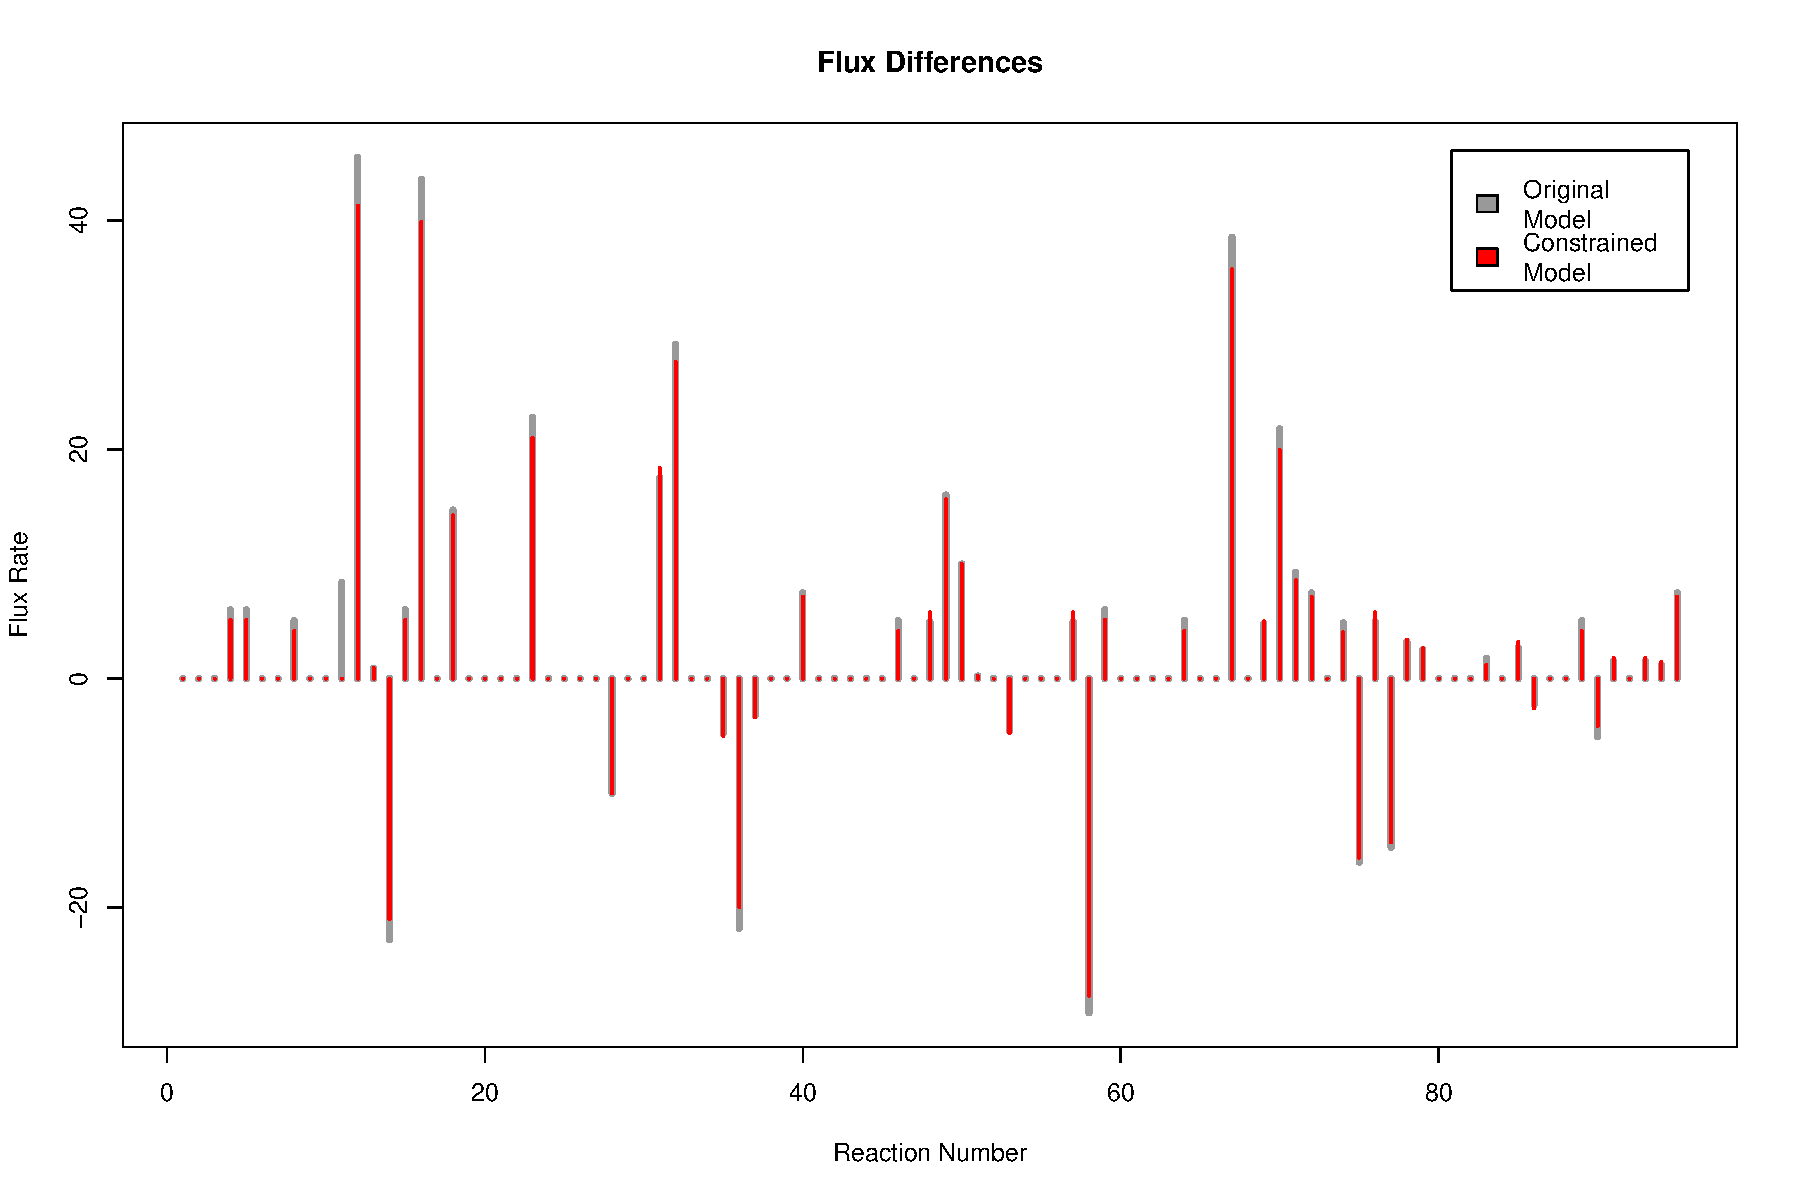
\includegraphics[width=0.5\textwidth]{exp2flux/exp2flux-001}\\
\caption{Flux differences between an unconstrained and a constrained model. Constraints were calculated through the \texttt{exp2flux} R package using simulated gene expression data.}
\label{exp2fluxFlux}
\end{center}
\end{figure}
\subsection*{Identifying flux changes between scenarios}
The measurement of flux change for each reaction between metabolic scenarios is a task generally carried out manually and oriented directly to the research objective. However, at system level analysis this process can become laborious. The \texttt{fluxDifferences} function calculates the fold change for each common reaction between metabolic scenarios. \emph{Fold change} is a measure that describes how much a quantity changes going from an initial to a final value. Implemented algorithm in the \texttt{fluxDifferences} functions are described in equation \ref{fC}, function takes as argument two valid models for the \texttt{`sybil'} R package and a customizable threshold value to filter functions to be reported.
\begin{align}
\label{fC}
\begin{split}
foldChange:&  \mathbb{R} \times \mathbb{R} \rightarrow \mathbb{R} \\
(rFluxModel1, rFluxModel2) \mapsto & \begin{cases}
rFluxModel2, & rFluxModel1 = 0; \\
\dfrac{(rFluxModel2 - rFluxModel1)}{\vert rFluxModel1\vert},  & \text{Other cases}
\end{cases}
\end{split}
\end{align}
As an example, we report the fold change of all reactions with an absolute change greatest or equal to 2-fold between the unconstrained and constrained metabolic scenarios simulated previously.
\begin{Schunk}
\begin{Sinput}
> fluxDifferences(
+   model1 = Ec_core,
+   model2 = mEc_core,
+   foldReport = 2
+   )
\end{Sinput}
\begin{Soutput}
           fluxModel1   fluxModel2 foldChange
ADK1     4.547474e-13 1.000444e-11         21
D_LACt2 -6.821210e-13 1.364242e-12          3
LDH_D   -6.821210e-13 1.364242e-12          3
\end{Soutput}
\end{Schunk}
\section{Summary}
We introduced the \textbf{exp2flux} package, an implementation of a previously described method to integrate gene-expression data in a continuous way into genome-scale metabolic network reconstructions. We show as an example, how the integration of a set of simulated data modifies the behavior of the \textit{E. coli} core metabolic model using Flux Balance Analysis simulations. Also, a example of the measurement of flux change between metabolic scenarios was showed.